\chapter{Association schemes}\label{association}
Association schemes arise in group theory, graph theory, design theory, coding theory and more. For example, if $X$ is a finite group with conjugacy classes $\cC[g] = \{hgh^{-1}:h\in X\}$ ($g\in X$), then the conjugacy class relations $R_g = \left\{ (a,b) \mid ab^{-1} \in \cC[g]  \right\}$ yield a 
commutative association scheme on the vertex set $X$. The orbits on $X\times X$ of any 
permutation group $G$ acting generously transitively on a set $X$  give a symmetric association scheme.
Some of the most well-studied association schemes are distance-regular graphs, including Moore graphs, distance-transitive graphs, strongly regular graphs, generalized polygons, etc. One studies 
$q$-ary error-correcting codes of length  $n$ as vertex subsets of the Hamming association scheme
$H(n,q)$ \cite[Sec.~9.2]{Brouwer1989} and one studies $t$-($v,k,\lambda$) designs as vertex subsets of the 
Johnson association scheme  $J(v,k)$ \cite[Sec.~9.1]{Brouwer1989}.  For an introduction to the 
extensive literature on the subject, the reader may consult \cite{Delsarte1973,Bannai1984,Brouwer1989,Godsil1993}, 
the survey \cite{Martin2009}, or the more recent book of  Bailey \cite{Bailey2005} which focuses on 
connections to the statistical design of experiments.

Let $X$ be a finite set of vertices. A \textit{symmetric d-class association scheme} (see \cite{Brouwer1989}) on $X$ is a pair $\mathcal{L} = (X,\mathcal{R})$ where $\mathcal{R} =\left\{R_0,R_1,\dots,R_d\right\}$ is a set of $d+1$ relations on $X$ satisfying the following properties:
\begin{enumerate}[label=(\roman*)]
	\item $R_0$ is the identity relation;
	\item $\left\{R_0,R_1,\dots, R_d\right\}$ forms a partition of $X\times X$;
	\item $(x,y)\in R_i$ implies $(y,x)\in R_i$;
	\item for $0\leq i,j,k\leq d$ there exist constants $p_{i,j}^k$ such that for any $(x,y)\in R_k$, the number of vertices $z$ for which $(x,z)\in R_i$ and $(z,y)\in R_j$ is equal to $p_{i,j}^k$ independent of our original choice of $x$ and $y$.
\end{enumerate}
The constants $p_{i,j}^k$ are known as the \emph{intersection numbers} of our association scheme and we allow ourselves to suppress the comma whenever $i$ and $j$ are given by single digits, thus $p_{0,7}^6$ and $p_{07}^6$ synonymous but we will never write $p_{102}^2$, instead using $p_{10,2}^2$. Property $(iii)$ and $(iv)$ together imply that $p_{ij}^k = p_{ji}^k$ for all $i,j,k$, thus any symmetric association schemes will be \textit{commutative}. There is a broader definition for an association scheme where we replace $(iii)$ with the requirement that for every $i$, there exists some $j$ such that $R_j = R_i^T$; that is $(x,y)\in R_i$ if and only if $(y,x)\in R_j$. In this case however, we add the additional requirement $p_{ij}^k = p_{ji}^k$ so that our scheme remains commutative. Throughout this text, all association schemes will be symmetric and therefore commutative, but we will add remarks at times when the theorems may be extended to the non-symmetric case.

For each $0\leq i\leq d$ we define the (undirected) graph $\Gamma_i = \Gamma(X,R_i)$ on $X$ with $\Gamma_1,\dots,\Gamma_d$ all simple. For each $a\in X$ we define the $i^\text{th}$ \emph{neighborhood} of $a$ $R_i(a) = \left\{b\in X\vert (a,b)\in R_i\right\}$; i.e. $R_i(a)$ is the neighborhood of $a$ in the graph $\Gamma_i$. Then for any $a\in X$, the set $X$ is partitioned into the \emph{subconstituents} $R_i(a)$ for $0\leq i\leq d$. Consider the following example on $8$ vertices:
\begin{example} Consider the association scheme called the \emph{3-cube} on vertex set $X = \left\{1,\dots,8\right\}$ with relations corresponding to the graphs $\Gamma_0,\dots,\Gamma_3$ given below in figure \ref{3cube}.\\
	\begin{figure}[H]\begin{center}\scalebox{.7}{$\begin{aligned}
	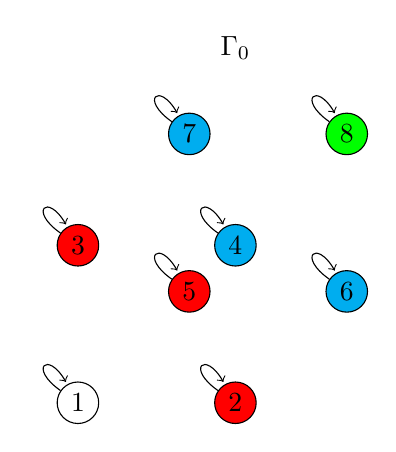
\begin{tikzpicture}[shorten >=1pt,auto,node distance=2cm,
	thin,main node/.style = {circle,draw, inner sep = 0pt, minimum size = 15pt}]
	
	\node[main node,fill=white] (1) {1};
	\node[main node,fill=red] [right of = 1](2) {2};
	\node[main node,fill=red] [above of = 1](3) {3};
	\node[main node,fill=cyan] [right of = 3](4) {4};
	\node[main node,fill=red] [above right of = 1](5) {5};
	\node[main node,fill=cyan] [right of = 5](6) {6};
	\node[main node,fill=cyan] [above of = 5] (7) {7};
	\node[main node,fill=green] [right of = 7](8) {8};
	\node at (2,4.5) (9) {$\Gamma_0$};
	
	\path (1) edge [in=120,out=145,loop] ();
	\path (2) edge [in=120,out=145,loop] ();
	\path (3) edge [in=120,out=145,loop] ();
	\path (4) edge [in=120,out=145,loop] ();
	\path (5) edge [in=120,out=145,loop] ();
	\path (6) edge [in=120,out=145,loop] ();
	\path (7) edge [in=120,out=145,loop] ();
	\path (8) edge [in=120,out=145,loop] ();
	
	\end{tikzpicture}\qquad&\qquad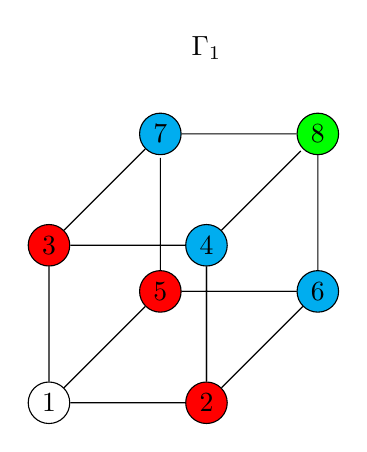
\begin{tikzpicture}[shorten >=1pt,auto,node distance=2cm,
	thin,main node/.style = {circle,draw, inner sep = 0pt, minimum size = 15pt}]
	\node[main node,fill=white] (1) {1};
	\node[main node,fill=red] [right of = 1](2) {2};
	\node[main node,fill=red] [above of = 1](3) {3};
	\node[main node,fill=cyan] [right of = 3](4) {4};
	\node[main node,fill=red] [above right of = 1](5) {5};
	\node[main node,fill=cyan] [right of = 5](6) {6};
	\node[main node,fill=cyan] [above of = 5] (7) {7};
	\node[main node,fill=green] [right of = 7](8) {8};
	\node at (2,4.5) (9) {$\Gamma_1$};
	
	\draw[-] (3)--(1)--(2)--(4)--(3)--(7)--(8)--(6)--(5)--(7);
	\draw[-] (1)--(5)--(6)--(2)--(4)--(8);
	\end{tikzpicture}\\\\
	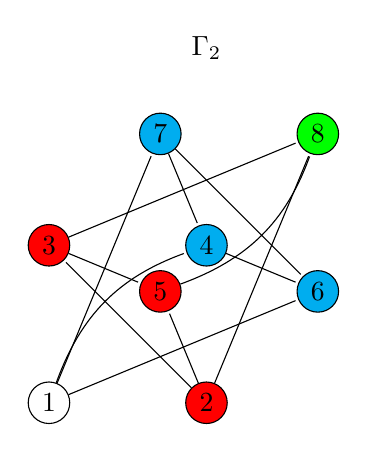
\begin{tikzpicture}[shorten >=1pt,auto,node distance=2cm,
	thin,main node/.style = {circle,draw, inner sep = 0pt, minimum size = 15pt}]
	\node[main node,fill=white] (1) {1};
	\node[main node,fill=red] [right of = 1](2) {2};
	\node[main node,fill=red] [above of = 1](3) {3};
	\node[main node,fill=cyan] [right of = 3](4) {4};
	\node[main node,fill=red] [above right of = 1](5) {5};
	\node[main node,fill=cyan] [right of = 5](6) {6};
	\node[main node,fill=cyan] [above of = 5] (7) {7};
	\node[main node,fill=green] [right of = 7](8) {8};
	\node at (2,4.5) (9) {$\Gamma_2$};
	
	\path[-]
	(1)edge [bend left=25] node {} (4)
	edge node {} (6)
	edge node {} (7)
	(2)edge node {} (3)
	edge node {} (5)
	edge node {} (8)
	(3)edge node {} (5)
	edge node {} (8)
	(4) edge node {} (6)
	(7) edge node {} (4)
	edge node {} (6)
	(5) edge [bend right = 25] node {} (8);
	\end{tikzpicture}\qquad&\qquad
	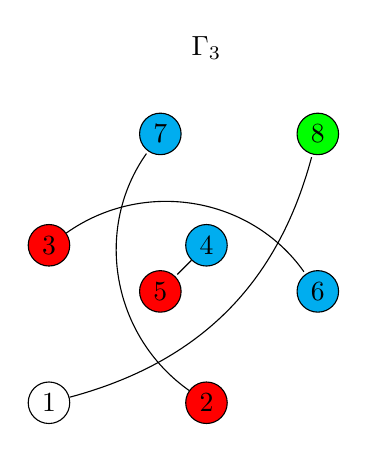
\begin{tikzpicture}[shorten >=1pt,auto,node distance=2cm,
	thin,main node/.style = {circle,draw, inner sep = 0pt, minimum size = 15pt}]
	\node[main node,fill=white] (1) {1};
	\node[main node,fill=red] [right of = 1](2) {2};
	\node[main node,fill=red] [above of = 1](3) {3};
	\node[main node,fill=cyan] [right of = 3](4) {4};
	\node[main node,fill=red] [above right of = 1](5) {5};
	\node[main node,fill=cyan] [right of = 5](6) {6};
	\node[main node,fill=cyan] [above of = 5] (7) {7};
	\node[main node,fill=green] [right of = 7](8) {8};
	\node at (2,4.5) (9) {$\Gamma_3$};
	
	\path[-]
	(1) edge [bend right] node {} (8)
	(2) edge [bend left=45] node {} (7)
	(3) edge [bend left=45] node {} (6)
	(4) edge node {} (5);
	\end{tikzpicture}
	\end{aligned}$}\end{center}
	\caption[Graphs of the 3-cube.]{The four graphs of the 3-cube. The four subconstituents of the vertex $1$ are colored white, red, blue, and green respectively.}\label{3cube}
	\end{figure}
	The intersection numbers of this association scheme are as follows, noting that $p^k_{ij} = p^k_{ji}$
	\[\begin{array}{c|cccc|ccc|cc|c}
	j & p^{j}_{0,0}	&p^{j}_{0,1}& p^{j}_{0,2} 	& p^{j}_{0,3}   & p^{j}_{1,1}	&p^{j}_{1,2}& p^{j}_{1,3} 	& p^{j}_{2,2} 	& p^{j}_{2,3} 	& p^{j}_{3,3}\\\hline
	0 & 1			& 0			& 0 			& 0				& 3				& 0			& 0 			& 3				& 0   			& 1\\
	1 & 0			& 1			& 0 			& 0				& 0				& 2			& 0 			& 0   			& 1   			& 0\\
	2 & 0			& 0			& 1 			& 0				& 2				& 0 		& 1				& 2 			& 0 			& 0\\
	3 & 0			& 0			& 0 			& 1				& 0 			& 3			& 0 			& 0   			& 0 			& 0\\
	\end{array}\]
\end{example}
For any $0\leq i\leq d$ and any vertex $x\in X$,
\[p^{0}_{ii} = \left\vert\left\{y:(y,x)\in R_i\right\}\right\vert = \left\vert R_i(x)\right\vert.\]
Thus we define $k_i:=p^0_{ii}$ as the \emph{valency} of the $i^\text{th}$ relation.
\begin{lem}{\cite[Lemma 2.1.1]{Brouwer1989}}\label{intrels}
	The parameters $k_i$, $p_{ij}^h$ of an association scheme with $d$ classes satisfy the following relations:
	\begin{enumerate}[label=(\roman*)]
		\item $p_{0j}^h = \delta_{jh}$,
		\item $p^0_{ij} = \delta_{ij}k_i$,
		\item $p^h_{ij} = p^h_{ji}$,
		\item $p^h_{ij}k_h = p^j_{ih}k_j$,
		\item $\sum_jp^h_{ij} = k_j$,
		\item $\sum_l p^l_{ij}p^m_{lh} = \sum_l p^m_{il}p^l_{jh}$.
	\end{enumerate}
\end{lem}
\begin{proof}
	Statements $(i)$ and $(ii)$ follow from our definition of the intersection numbers and the requirement that $R_0$ is the identity relation. We have already shown that $(iii)$ follows from the symmetric property. To show $(iv)$, consider a fixed point $x$ and the subconstituents $R_k(x)$ and $R_j(x)$. Counting the number of edges in $\Gamma_i$ between $R_k(x)$ and $R_j(x)$ in two different ways gives our result. For $(v)$ consider that for $(x,y)\in R_k$,
	\[\sum_{j}p_{ij}^k = \left\vert R_i(x)\cap\left(\bigcup_{j=0}^dR_j(y)\right)\right\vert = \left\vert R_j(y)\right\vert.\]
	Finally $(vi)$ may be shown by counting quadruples $(x,y,z,w)$ with $(x,y)\in R_i$, $(y,z)\in R_j$, and $(z,w)\in R_k$ for a fixed pair $(x,w)\in R_m$.
\end{proof}
\section{Bose-Mesner algebra}
Often it becomes useful to order the vertices in $X$ and then represent each $R_i$ as a 01-matrix $A_i$ where the $(x,y)$ entry of $A_i$ is 1 if and only if $(x,y)\in R_i$, thus $A_i$ is the adjacency matrix of $\Gamma_i$. The defining properties of an association scheme are then encoded as:
\begin{enumerate}[label=(\roman*)]
	\item $A_0 = I$;
	\item $\sum_i A_i = J$;
	\item for all $0\leq i\leq d$, $A_i^T = A_i$;
	\item for all $0\leq i,j\leq d$, $A_iA_j = \sum p_{i,j}^k A_k$.
\end{enumerate}
The fourth condition tells us that $\BMA = \text{span}\left\{A_0,A_1,\dots A_d\right\}$ forms a matrix algebra under standard matrix multiplication. We call this algebra the \emph{Bose-Mesner algebra} and note that the remaining conditions ensure it is a $(d+1)$-dimensional algebra of symmetric matrices containing the identity. Further, as our basis matrices are 01-matrices with disjoint support, this algebra is also closed under Schur (element-wise) products. Since $p^k_{ij} = p^k_{ji}$ for all $i,j,k$, we must have $A_iA_j = A_jA_i$, that is our algebra is also commutative. Therefore we may simultaneously diagonalize the matrices $\left\{A_0,\dots,A_d\right\}$ using the maximal common orthogonal eigenspaces $V_0,\dots,V_{d'}$ with corresponding idempotents $E_0,\dots,E_{d'}$. Since, for every $i$, there exists eigenvalues $\theta_{ij}$ such that $A_i = \sum_{j=0}^{d'}\theta_{ij}E_j$ we find that $\BMA \subseteq \text{span}\left\{E_0,E_1,\dots, E_{d'}\right\}$ thus $d\leq d'$. Further since the eigenspaces $V_j$ are maximal for each $0\leq j\leq d$ and pairwise orthogonal,
\[E_j = \frac{1}{c_j}\prod_{i=0}^d\left(\prod_{\theta_{ik}\neq\theta_{ij}}\left(A_i-\theta_{ik}I\right)\right)\]
for some normalization constant $c_j$. Thus $E_j\in \BMA$ giving $\text{span}\left\{E_0,E_1,\dots, E_{d'}\right\}\subseteq\BMA$ and therefore $d=d'$. Then, for any $d$-class association scheme there is a basis of exactly $d+1$ idempotents $E_0,\dots,E_d$ which are unique up to reordering and diagonalize every matrix in $\BMA$. Since $J\in\BMA$, the rank 1 idempotent $\frac{1}{\vert X\vert}J$ must be contained within this basis; by convention we assume $E_0= \frac{1}{\vert X\vert}J$. For each $0\leq j\leq d$ we denote the rank of $E_j$ as $m_j$ and note that $E_iE_j = \delta_{ij}$. As both $\left\{A_0,\dots,A_d\right\}$ and $\left\{E_0,\dots,E_d\right\}$ form bases for the Bose-Mesner algebra, there exists unique matrices $P$ and $Q$ so that
\begin{equation}
\label{PQmat}
A_i = \sum_{j} P_{ji} E_j,\qquad E_j = \frac{1}{\vert X\vert} \sum_{i} Q_{ij}A_i.
\end{equation}
We call $P$ and $Q$ the first and second eigenmatrices, noting that the eigenvalues of $A_i$ are given by column $i$ of $P$ and the entries of $\vert X\vert E_j$ are given by column $j$ of $Q$. We again refer to \cite{Brouwer1989} for the following lemma concerning the first and second eigenmatrices
\begin{lem}{\cite[Lemma 2.2.1]{Brouwer1989}}\label{PQrels} The matrices $P$ and $Q$ of an association scheme satisfy:
	\begin{enumerate}[label=(\roman*)]
		\item $P_{j0} = 1$, $Q_{i0} = 1$,
		\item $P_{0i} = k_i$, $Q_{0j} = m_j$,
		\item $P_{ij}P_{jh} = \sum_lp^l_{jh}P_{il}$,
		\item $m_jP_{ji} = k_iQ_{ij},\qquad\sum_j m_jP_{ji}P_{jh} = \vert X\vert k_i\delta_{jh},\qquad\sum_j k_iQ_{ij}Q_{ih} = \vert X\vert m_j\delta_{jh}$,
		\item $P_{ji}Q_{hj} = \sum_lp_{il}^hQ_{lj}$,
		\item $\vert P_{ji}\vert\leq k_i,\qquad\vert Q_{ij}\vert\leq m_j$,
		\item $\sum_{j}P_{ji} = \sum_{h}p^h_{hi}$.\qed
	\end{enumerate}
\end{lem}
In particular let $\Delta_m=\text{diag}(m_0,m_1,\dots,m_d)$ and $\Delta_k=\text{diag}(k_0,k_1,\dots,k_d)$ and the following two relations hold for our eigenmatrices:
\begin{lem}[\cite{Brouwer1989}, First and second orthogonality relations] The matrices $P$ and $Q$ of an association scheme satisfy:
	\begin{equation}
		PQ = \vert X\vert I, \qquad \Delta_mP = Q^T\Delta_k
	\end{equation}
\end{lem}
\begin{proof}
	First consider that for all $0\leq j\leq d$,
	\[E_j = \frac{1}{\vert X\vert}\sum_i Q_{ij}A_i = \frac{1}{\vert X\vert}\sum_i \sum_{j} Q_{ij}P_{ji} E_j\]
	Thus $\frac{1}{\vert X\vert}\sum_i \sum_{j} Q_{ij}P_{ji} = \delta_{ij}$. The second orthogonality relation is given by Lemma \ref{PQrels} $(iv)$.
\end{proof}
As $\BMA$ is closed under Schur products, we find that there exist structure constants $q_{i,j}^k$ such that for all $0\leq i,j\leq d$:
\begin{equation}E_i\circ E_j = \frac{1}{\vert X\vert}\sum_k q_{i,j}^k E_k.\label{Emult}\end{equation}
We call these parameters the \emph{Krein parameters} of the association scheme. We quickly find properties analogous to those of the intersection numbers listed in Lemma \ref{intrels}.
\begin{lem}{\cite[Lemma 2.3.1]{Brouwer1989}}\label{kreinrels} The parameters $m_j$, $q_{ij}^k$ of an association scheme with $d$ classes satisfy the following relations:
	\begin{enumerate}[label=(\roman*)]
		\item $q^k_{0j} = \delta_{jk}$,
		\item $q^0_{ij} = \delta_{ij}m_j$,
		\item $q^{k}_{ij} = q^k_{ji}$,
		\item $q^k_{ij}m_k = q^j_{ik}m_j$,
		\item $\sum_j q^k_{ij} = m_i$,
		\item $\sum_l q^l_{ij}q^{m}_{lk} = \sum_lq^m_{il}q^l_{jk}$,
		\item $Q_{ij}Q_{ik} = \sum_{l}q^l_{jk}Q_{il}$,
		\item $P_{ki}Q_{ij} = \sum_l q^k_{jl}P_{li}$.\qed
	\end{enumerate}
\end{lem}
\section{Feasibility conditions}
We are often interested in determining whether an association scheme exists given a parameter set. While we often cannot guarantee existence without finding the entire scheme, there are many times where we may rule out a parameter set due to its intersection numbers or Krein parameters. In this section we examine three main conditions which we will use throughout this text. We first begin with the intersection numbers:
\begin{lem}[\cite{Brouwer1989}]\label{intfeas}
	The intersection numbers of an association scheme must be non-negative integers.
\end{lem}
This condition is easy to verify since, by definition, each $p^k_{ij}$ must be the cardinality of a set.
\begin{example}
	There is no strongly regular graph (association scheme with two non-trivial relations) on 10 vertices with $k_1 = 5$ and $p^1_{12}=3$. Since $k_0+k_1+k_2 =\vert X\vert =10$ we must have $k_2=4$ in this case, but then $p^2_{12} = \frac{k_1}{k_2}p^1_{12} = \nicefrac{15}{4}\notin\bbZ$ and feasibility condition 1 is violated.
\end{example}
Now consider the Krein parameters of our association scheme.
\begin{lem}[\cite{Scott1973},Krein conditions]\label{kreinfeas}
	The Krein parameters of an association scheme must be non-negative real numbers.
\end{lem}
\begin{proof}
	From equation \eqref{Emult}, we find that $\frac{q_{ij}^0}{\vert X\vert},\dots,\frac{q_{ij}^d}{\vert X\vert}$ are the eigenvalues of $E_i\circ E_j$. However $E_i\circ E_j\in BMA$ and thus it must be symmetric and therefore all eigenvalues are real. Further, $E_i\circ E_j$ is a principle submatrix of $E_i\otimes E_j$, which has two distinct eigenvalues: $1$ and $0$. Therefore $E_i\otimes E_j$ is positive semi-definite and any principle submatrix must share the same property, forcing the eigenvalues of $E_i\circ E_j$ to be non-negative.
\end{proof}
The final feasibility condition we will list here is known as the \emph{absolute bound}.
\begin{lem}[\cite{Neumaier1981},Absolute bound]\label{absolute}
	The multiplicities $m_i$ ($0\leq i\leq d$) of a $d$-class association scheme satisfy:
	\[\sum_{q_{ij}^k\neq 0} m_k\leq\begin{cases}
	m_im_j & \text{ if }i\neq j\\
	\binom{m_i+1}{2} & \text{ if }i= j.
	\end{cases}\]
\end{lem}
\begin{proof}
	The sum on the left is the rank of $E_i\circ E_j$, a principle submatrix of $E_i\otimes E_j$ which has rank $m_im_j$. If $i=j$, $E_i\circ E_i$ is the entrywise square of $E_i$. Assume $\text{col}(E_i) = \text{span}(v_1,\dots,v_{m_i})$, then the columns of $E_i\circ E_i$ must be linear combinations of the vectors $v_j\circ v_k$ for $1\leq j\leq k\leq d$, a total of $\binom{m_i+1}{2}$ vectors.
\end{proof}
\begin{definition}
	A \emph{feasible parameter set} is a set of Krein parameters and intersection numbers such that:
	\begin{itemize}
		\item[FC1:] The Krein parameters satisfy Lemmas \ref{kreinfeas} and \ref{kreinrels},
		\item[FC2:] The intersection numbers satisfy Lemmas \ref{intfeas} and \ref{intrels},
		\item[FC3:] For $m_j = q^0_{jj}$, the integers $0\leq m_j\leq d$ satisfy Lemma \ref{absolute}.
	\end{itemize}
\end{definition}
\section{Parameter arrays}
For a matrix $A$, we denote the entry in row $i$ and column $j$ as $\left[A\right]_{ij}$. We then define the \emph{arrays of intersection numbers} $L_0,\dots,L_d$ as $(d+1)\times(d+1)$ matrices where $\left[L_i\right]_{k,j} = p^k_{ij}$. We then define the vector space $\bbL = \text{span}\left\{L_0,\dots,L_d\right\}$ and note that Lemma \ref{intrels} $(vi)$ gives us that
\[
	\left[L_iL_j\right]_{m,k} = \sum_lp^m_{il}p^l_{jk} = \sum_{l}p^l_{ij}p^m_{lk} = \sum_l p^l_{ij}\left[L_l\right]_{m,k}
\]
for $0\leq m,k\leq d$. Therefore we find that this vector space forms a matrix algebra under matrix multiplication via
\begin{equation}\label{Lprod}
	L_iL_j = \sum_l p^l_{ij}L_l
\end{equation}
extended linearly. We therefore may define an algebra isomorphism $\phi:\BMA\rightarrow\bbL$ via the basis mapping $\phi(A_i) = L_i$. Note that this isomorphism preserves standard matrix multiplication, however entrywise multiplication need not be preserved. Likewise we define the \emph{arrays of Krein parameters} as $L_0^*,\dots,L_d^*$ with $\left[L_i^*\right]_{k,j} = q^k_{ij}$. This provides a dual vector space $\bbL^* = \text{span}\left\{L_0^*,\dots,L_d^*\right\}$ with Lemma \ref{kreinrels} $(vi)$ giving
\begin{equation}\label{Lstarprod}
	L_i^*L_j^* = \sum_{l}q^l_{ij}L_l^*.
\end{equation}
We then define a second algebra isomorphism, this time mapping entrywise products to matrix multiplication, $\phi^*:\BMA\rightarrow\bbL^*$ via the basis mapping $\phi^*(E_i) = \frac{1}{\vert X\vert}L_i^*$. We call $L_1$ the \emph{intersection matrix} and $L_1^*$ the \emph{Krein matrix} as these two matrices will become especially important for polynomial schemes (see Section \ref{ppoly} and \ref{qpoly}).
\section{Imprimitivity}
\section{Metric schemes}\label{ppoly}
\section{Cometric schemes}\label{qpoly}
A \textit{$Q$-polynomial} (\textit{cometric}) association scheme is one in which the set $\left\{E_0,E_1,\dots,E_d\right\}$ may be ordered so that $q^{k}_{i,j} = 0$ whenever $k>i+j$ or $k<\vert i- j\vert$ and $q^{k}_{i,j}>0$ whenever $k = i+j$. Finally, we say an association scheme with $Q$-polynomial ordering $E_0,\dots,E_d$ is \textit{$Q$-antipodal} if $q^{k}_{d,d} >0$ when $k = 0$ but $q^{k}_{d,d} = 0$ for $0<k<d$. Given a $Q$-polynomial ordering $E_0,\dots,E_d$ we find it convenient to order relations so that $Q_{01}>Q_{11}>\dots>Q_{d1}$; we call this the natural ordering. We call these parameters the Krein parameters of the association scheme. We conclude this section by examining the Krein parameters of our scheme, and defining an algebra isomorphism from our Bose-Mesner algebra to a new matrix algebra. Defining $L_i^*$ such that
\[L_i^* = [q^k_{i,j}]_{k,j},\]
we may define the vector space $\mathbb{L}^* = \text{span}\left\{L_0^*,L_1^*,\dots,L_d^*\right\}$. From \cite[Lemma.~2.3.1(vi)]{Brouwer1989}, we have:
\begin{align}
L_i^*L_j^* = \sum_k q^m_{i,k}q^k_{j,l}&=\sum_k q^k_{i,j}q^m_{k,l}=\sum_{k}q^k_{i,j}L_k^*,\label{dblsum}\end{align}
showing that $\mathbb{L}^*$ is closed under matrix multiplication. Therefore we define a homomorphism $\phi^* : \mathbb{A}\rightarrow \mathbb{L}^*$ via taking $\phi^*(E_i) = \frac{1}{\vert X\vert}L_i^*$ for each $0\leq i\leq d$ and extending linearly. From \eqref{dblsum}, we see that
\[\phi^*(E_i\circ E_j) = \frac{1}{\vert X\vert}\sum_{k=0}^{d}q^k_{i,j}\phi^*\left(E_k\right) = \frac{1}{\vert X\vert^2}\sum_{k=0}^dq^k_{i,j}L_k^* = \left(\frac{1}{\vert X\vert}L_i^*\right)\left(\frac{1}{\vert X\vert}L_j^*\right) = \phi^*(E_i)\phi^*(E_j).\]
Therefore $\phi^*$ is an algebra isomorphism preserving the Schur product structure of $\mathbb{A}$.
\section{Strongly regular graphs--2-class association schemes}
A strongly regular graph with parameters $(v,k,\lambda,\mu)$ is a $k$-regular graph with $v$ points where every pair of adjacent (non-adjacent) vertices have exactly $\lambda$ ($\mu$) neighbors in common. Thus, a strongly regular graph $\Gamma$ corresponds to $2$-class association scheme where $\Gamma$ and $\overline{\Gamma}$ are the two non-trivial relations. Thus a 2-class association scheme has the following first and second eigenmatrices:
\begin{equation}\label{PQsrg}P = \left[\begin{array}{ccc}
1 & k & v-k-1\\
1 & r & -(r+1)\\
1 & s & -(s+1)
\end{array}\right]\qquad Q = \left[\begin{array}{ccc}
1 & f & g\\
1 & \frac{fr}{k} & \frac{gs}{k}\\
1 & \frac{f(1+r)}{k+1-v} & \frac{g(1+s)}{k+1-v}
\end{array}\right]\end{equation}
where $\Gamma$ has spectrum $k^1,r^f,s^g$. The following are two theorems which will prove useful later.
\begin{thm}\cite[Theorem.~1.3.1.(iii)]{Brouwer1989} Whenever $\mu>0$, the parameters of a strongly regular graph may be expressed in terms of $r$, $s$, and $\mu$ as
	\[k = \mu-rs, \qquad v = \frac{(k-r)(k-s)}{\mu},\qquad \lambda = \mu+r+s.\]
\end{thm}
\begin{thm}\cite{Delsarte1973} 
	Let $\Gamma$ be a strongly regular graph with $v$ vertices, valency $k$, and smallest eigenvalue $-m$. If $C$ is a coclique of $\Gamma$, then
	\[\vert C\vert\leq v\left(1+\frac{k}{m}\right))^{-1}, \]
	with equality if and only if every vertex $\gamma\notin C$ has the same number of neighbors (namely $m$) in $C$.
\end{thm}
\section{Cometric Association Schemes}
Let $(X,\mathcal{R})$ be an $d$-class symmetric association scheme. We say $(X,\mathcal{R})$ is $Q$-polynomial, or \textit{cometric}, if there exists an ordering of the eigenspaces, say $E_0$, $E_1$,\dots, $E_d$, such that the Krein parameters satisfy the following conditions:
\begin{enumerate}
	\item $q^k_{i,j} = 0$ whenever $i+j<k$, and
	\item $q^{i+j}_{i,j}>0$ whenever $i+j\leq d$.
\end{enumerate}
Under these conditions, we see that for a given $0\leq j\leq d$, at most three possible choices for $k$ will allow $q_{1,k}^j>0$. Therefore let $c_j^* = q_{1,j-1}^j$, $a_j^* = q_{1,j}^j$ and $b_j^* = q_{1,j+1}^j$ for $0\leq j\leq d$ with the restriction that $b_d^*=c_0^*=0$. Given a cometric scheme, we define the Krein array as $\left\{b_0^*,b_1^*,\dots,b_{d-1}^*;c_1^*,c_2^*,\dots,c_d^*\right\}$ noting that for any $0\leq j\leq d$, $c_j^* + a_j^* + b_j^* = q^0_{1,1}$. We say a cometric scheme is $Q$-\emph{bipartite} if $a_j^*=0$ for all $0\leq j\leq d$. This is equivalent to the condition that $q_{i,j}^k=0$ whenever $i+j+k$ is odd. A cometric scheme is $Q$-\emph{antipodal} if $b_j^* = c_{d-j}^*$ for all $j$ except possibly $j = \lfloor \frac{d}{2}\rfloor$.\par
We may define orthogonal polynomials $q_j(t)$, $j=0,1,\dots,d$ by $q_0(t) = 1$, $q_1(t) = t$ and the three-term recurrence $tq_j(t) = c_{j+1}^*q_{j+1}(t) + a_j^*q_j(t) + b_{j-1}^*q_{j-1}(t)$. It follows that $\vert X\vert E_j = q_j(\vert X\vert E_1)$, for $j=0,1,\dots,d$ where matrix multiplication is computed entrywise. Since $\frac{1}{\vert X\vert}Q_{i,j}$ for $0\leq i\leq j$ are the entries of $E_j$, this also means that $q_j(Q_{i,1}) = Q_{j,1}$. Finally note that in the $Q$-bipartite case, $q_j(t)$ is an even polynomial if and only if $j$ is even.\par
The following two theorems will help us describe the quotient object we find in the $Q$-bipartite case where $I_r$ and $J_r$ denote the $r\times r$ identity and all ones matrix respectively:
\begin{thm}[\cite{Martin2007}] \label{mmw}The following are equivalent:
	\begin{enumerate}[label=(\roman*)]
		\item $(X,\mathbb{R})$ is imprimitive;
		\item for some $j>0$, $E_j$ has repeated columns;
		\item for some subset $\mathcal{I} = \left\{i_0=0,i_1,\dots,i_s\right\}$ of $\left\{0,1,\dots,d\right\}$ and some ordering of the vertices $\sum_{h=0}^s A_{i_h} = I_w\otimes J_r$ for integers $w$ and $r$ with $\vert X\vert=wr$, $1<w,r<\vert X\vert$;
		\item for some subset $\mathcal{J} = \left\{j_0=0,j_1,\dots,j_s\right\}$ of $\left\{0,1,\dots,d\right\}$ and some ordering of the vertices $\sum_{h=0}^s E_{j_h} = \frac{1}{r}\left(I_w\otimes J_r\right)$ for integers $w$ and $r$ with $\vert X\vert=wr$, $1<w,r<\vert X\vert$.
	\end{enumerate}
\end{thm}
Whenever $(iii)$ occurs, say with subset $\mathcal{I}$ as given in the theorem, we may partition our vertices into equivalence classes so that $x\sim y$ whenever $(x,y)\in R_i$ for some $i\in \mathcal{I}$. Let $X_1,\dots,X_w$ be the corresponding equivalence classes and define $\mathcal{R}' = \left\{R_i\in \mathcal{R} : i\in \mathcal{I}\right\}$. Then there exists \emph{subschemes} $(X_i,\mathcal{R}')$ for each equivalence class $X_i$. Further, we may define a \emph{quotient scheme} $(\tilde{X},\tilde{\mathcal{R}})$ of our original scheme with respect to $\mathcal{I}$ whose point set is the set of equivalence classes and whose relations are $R_{\tilde{i}} = \cup_{i\in \tilde{i}} R_i$ where each $\tilde{i} = \left\{0\leq j\leq d : p^x_{i,j} \text{ for }x\in \mathcal{I}\right\}$. Note that $\vert \tilde{\mathcal{R}}\vert = \vert \mathcal{J}\vert$ where $\mathcal{J}$ is the subset from Theorem $3.1(iv)$.
\begin{thm}[\cite{Suzuki1998}] \label{suzuki}Suppose $(X,\mathcal{R})$ is an imprimitive cometric association scheme. Then one of the following holds:
	\begin{enumerate}[label=(\roman*)]
		\item $(X,\mathcal{R})$ is $Q$-bipartite and $\mathcal{J} = \left\{0,2,4,\dots\right\}$
		\item $(X,\mathcal{R})$ is $Q$-antipodal and $\mathcal{J} = \left\{0,d\right\}$
		\item $(X,\mathcal{R})$ is a $4$-class scheme with Krein array $\left\{m,m-1,1,b_3^*;1,c_2^*,m-b_3^*,1\right\}$ and $\mathcal{J} = \left\{0,3\right\}$;
		\item $(X,\mathcal{R})$ is a $6$-class scheme with Krein array $\left\{m,m-1,1,b_3^*,b_4^*,1;1,c_2^*,m-b_3^*,1,c_5^*,m\right\}$ and $\mathcal{J} = \left\{0,3,6\right\}$.
	\end{enumerate}
\end{thm}
Cerzo and Suzuki \cite{Cerzo2009} have shown that no association schemes of the third type exist.
\begin{cor}
	\label{SRG}
	The quotient scheme of a 4-class $Q$-bipartite association scheme is a strongly regular graph.
\end{cor}
\begin{proof}
	From Theorem \ref{suzuki}, we know $\mathcal{J} = \left\{0,2,4\right\}$ and therefore the quotient scheme has two nontrivial relations, forcing it to be strongly regular.
\end{proof}
\begin{thm}[\cite{Brouwer2003},\cite{Martin2007}]
	\label{sym}
	If $(X,\mathcal{R})$ is $Q$-bipartite with $w$ dual bipartite classes of size $r$ each, then $r=2$. Under the natural ordering of relations, $\mathcal{I} = \left\{0,d\right\}$ and the sequence $m = Q_{01}>Q_{11}>\dots>Q_{d1}$ is symmetric about the origin. In particular, $Q_{\frac{d}{2},1} = 0$ whenever $d$ is even.
\end{thm}
\begin{cor}
	\label{evenpoly}
	If $(X,\mathcal{R})$ is $Q$-bipartite, then $Q_{i,j} = Q_{d-i,j}$ $(-Q_{d-i,j}$, resp.) whenever $j$ is even (odd).
\end{cor}
\begin{proof}
	$q_j(t)$ is even (odd) whenever $j$ is even (odd). Since $Q_{i,1} = -Q_{d-i,1}$ and $Q_{i,j} = q_j(Q_{i,1})$, the result follows.
\end{proof}

Let $(X,\cR)$ be a commutative $d$-class association scheme with \emph{basis relations}
$\cR=\{R_0,$ $\ldots,R_d\}$. For $1\le  i\le d$, we have
a (possibly directed) simple graph $\Gamma_i=(X,R_i)$ on $X$. For $a\in X$, the set $X$ is partitioned into \emph{subconstituents} $R_i(a) = \{ b\in X \mid (a,b)\in R_i \}$ ($0\le i\le d$) with respect to $a$. The association
scheme is \emph{symmetric} if all basis relations are symmetric; each $\Gamma_i$ may be considered as an
undirected graph in this case as $i'=i$ for all $i$. The association scheme  is \emph{primitive} 
\cite[Sec.~2.4]{Brouwer1989} if $\Gamma_i$ is connected for all $i=1,\ldots, d$ and \emph{imprimitive} otherwise. A 
\emph{system of imprimitivity} for $(X,\cR)$ is any non-trivial partition of $X$ consisting of the components of
some graph $(X,R)$ where $R$ is a union of basis relations. (The trivial partitions  $\{X\}$ and 
$\{ \{a\} \mid a\in X\}$ are not systems of imprimitivity.)
For each $i$, we  may construct  an undirected graph $H_i$ (possibly with loops) on vertex set 
$\{0,1,\ldots,d\}$, joining  $j$ to $k$ if $p_{ij}^k+p_{ik}^j > 0$. 
We call this the \emph{unweighted distribution diagram} corresponding to basis relation $R_i$.
%%%%%%%%%%%%  JUNE 16
%%%%%%%%%%%%
%%%%%%%%%%%% Check definition of H_i when scheme is not symmetric.

With reference to a fixed undirected graph $\Gamma$ % on $X$ 
with vertex set $V\Gamma$ and edge 
set $E\Gamma$,  we say that $a$ and $b$ are \emph{twins} if $a\neq b$ yet
$\Gamma(a)=\Gamma(b)$, where $\Gamma(a)$ denotes the set of neighbors of $a$ in graph $\Gamma$.
Write\footnote{Note that some authors assign another meaning to $\bot$; here, we follow \cite[p.\ 440]{Brouwer1989}.} 
$a^\bot = \{a \} \cup \Gamma(a)$. A graph $\Gamma$ is \emph{complete multipartite} if any two
non-adjacenct vertices are twins: i.e., the complement of $\Gamma$ is a union of complete graphs.